\documentclass[12pt, oneside, a4paper]{book}

\usepackage[pdftex]{graphicx}
\usepackage{tikz-cd}
\usepackage{bm}
\usepackage{amsmath}
\usepackage{amssymb}
\usepackage{amsthm}
\usepackage{pgfplots}
\usepackage{xcolor}
\usepackage[shortlabels]{enumitem}
\usepackage[mathscr]{euscript}
\pgfplotsset{compat = newest}

\usepackage{vuwproposal} % sets up some local things, mostly the front page

\usepackage{palatino} % sets palatino as the default font

\usepackage{url} % for typesetting urls



%\renewcommand{\baselinestretch}{1.00}


\begin{document} 
	
	
\frontmatter
% Book style knows about front matter
% Report style doesn't so you need to set roman numbering etc yourself :-(

%%%%%%%%%%%%%%%%%%%%%%%%%%%%%%%%%%%%%%%%%%%%%%%%%%%%%%%
	
\title{New Features of Permutation Entropy in Ordinal Patterns Complexity Plane}
%%% ACF Correct the title

\author{Rasika Dilhani}
\supervisor{Alejandro C.\ Frery}
	
\subject{Data Science}
\abstract{This proposal provides a brief introduction to ordinal patterns and a literature review related to the Bandt \& Pompe research article. 
After reviewing the literature on ordinal patterns and permutation entropy, 
%%% ACF Didn't you consider the Complexity?
we can conclude that ordinal patterns play an important role in conducting research. 
Bandt \& Pompe proposed analyzing time series from the perspective of ordinal patterns to develop fast and automated methods for extracting qualitative information from nonlinear time series. 
They introduced the concept of permutation entropy to measure the complexity 
%%% ACF The sentence above may confuse the reader: does the PE measure the complexity?
of a system underlying a time series while taking into account the ordering patterns that represent variations in the data. 
In this report I show how to use data to extract all ordinal patterns. 
%%% ACF You show more than the mere extraction
First, I use the sample dataset to calculate their ordinal patterns with embedding dimension 3; 
%%% ACF The reader doesn't know what the embedding dimension is
I use letters to convert time series data into patterns.
Secondly, I get the histogram on the data. 
%%% ACF No, you don't; you compute the histogram of symbols
And third, calculate the permutation entropy and statistical complexity. 
Next, determine the confidence interval of H 
%%% ACF Always use mathematical notation. What is H? What is this time dependence?
without and with time dependence and finally the confidence interval of C.
		
Bandt and Pompe's ordinal pattern methodology has been widely used to investigate the latent dynamics of time series through their entropy, also known as permutation entropy. 
Nevertheless, there are no theoretical findings regarding the distribution of the permutation entropy, which needs to take the correlation effect between patterns into account. 
Considering that our approximation ignores the series dependence between symbols and that the asymptotic distribution of the permutation entropy is Normal %\cite{Rey2023}, \cite{Rey2023a}%. 
%%% ACF The sentence above is incomplete. What is "your" approximation?
%%% ACF In the sentence below, what is the "multinomial sample entropy"?
We compare this result with the Multinomial sample entropy with embedding dimension 3, which assumes independence, and find that the expression of the asymptotic variance becomes more complex as the embedding dimension increases. 
After that, a hypothesis test is developed and used to differentiate between the bearing fault diagnoses for four distinct rotating machines.}	
%%% ACF Do you differentiate "bearing fault diagnoses"?

% Books don't normally have abstracts, and this is a bit of a hack
	
% Uncomment the appropriate degree
\phd
%\mscthesisonly
%\mscwithhonours
%\mscbothparts
% \otherdegree{DEGREE OR DIPLOMA NAME}
	
	
	
%%%%%%%%%%%%%%%%%%%%%%%%%%%%%%%%%%%%%%%%%%%%%%%%%%%%%%%
%New commands:
	
\newcommand{\Sha}{\rotatebox[origin=c]{180}{$\Pi\kern-0.361em\Pi$}}
\newcommand{\ot}{\otimes}
\newtheorem{definition}{Definition}
\newtheorem{theo}{Theorem}
\newtheorem{contoh}{Example}
\newtheorem{cor}{Corollary}
\newtheorem{prop}{Proposition}
\newtheorem{lemma}{Lemma}
\newtheorem{remark}{Remark}
\newtheorem{conjecture}{Conjecture}
%%%%%%%%%%%%%%%%%%%%%%%%%%%%%%%%%%%%%%%%%%%%%%%%%%%%%%%
	
\maketitle
	
%\chapter*{Acknowledgments}\label{C:ack} 

Any acknowledgments should go in here, between the title page and the
table of contents.  The acknowledgments do not form a proper chapter,
and so don't get a number or appear in the table of contents.
	
\tableofcontents
	
	
%%%%%%%%%%%%%%%%%%%%%%%%%%%%%%%%%%%%%%%%%%%%%%%%%%%%%%%
	
% book style knows about mainmatter
% if you are using report style you will have to rest page numbering etc.
\mainmatter
	
%%%%%%%%%%%%%%%%%%%%%%%%%%%%%%%%%%%%%%%%%%%%%%%%%%%%%%%
	
% individual chapters included here
	
\chapter{Introduction}\label{C:intro}

This proposal presents the use of permutation entropy 
%%% ACF Won't you use the complexity?
and ordinal patterns in time series analysis, including the calculation of pattern histograms, entropy, and complexity to better understand their statistical properties. 
Additionally, the confidence intervals for entropy and
%%% ACF Capitalize distributions: Multinomial
complexity under the multinormal distribution and features for time series clustering are discussed. 
The concept of ordinal patterns in time series was introduced by Bandt and Pompe \cite{PhysRevLett.88.174102}. This study focuses on features derived from Bandt \& Pompe symbolization, specifically Shannon entropy. 
%%% ACF Why not the complexity?
Future work will extend to other measures, such as Rényi entropy, Fisher information, and the confidence intervals for their entropy and complexity under the multinormal distribution. Features for time series clustering 
%%% ACF Not within, but with
within ordinal patterns for time series analysis will be further studied.

Time series analysis is widely applied across various fields, including engineering, economics, physical sciences, and more. A time series is defined as a collection of observations ${x_t}$, each representing a realized value of a particular random variable $X_t$, where time can be either discrete or continuous.

Examples of time series applications include finance (e.g., analyzing exchange rate movements or commodity prices), biology (e.g., modeling the growth and decline of bacterial populations), medicine (e.g., tracking the spread of diseases like COVID-19 or influenza), and geoscience (e.g., predicting wet or dry days based on past weather conditions).

The primary goal of time series analysis is to understand the nature of the phenomenon represented by the observed sequence. Time domain and frequency domain methods are the two primary approaches used in time series analysis. The temporal approach relies on concepts such as auto-correlation and regressions, where a time series' present value is analyzed in relation to its own past values or the past values of other series. This method represents time series directly as a function of time. On the other hand, the spectral approach represents time series through spectral expansions, such as wavelets or Fourier modes~\cite{treitel1995spectral}.
%%% ACF You don't have this reference in the BibTeX database
 
%%% ACF Spectral, temporal or both? Citation 
However, these methods often require assumptions such as large sample sizes or normally distributed observations that are rarely met in real-world empirical data. For many statistical techniques to be valid, these assumptions must hold, but in practice, they are frequently violated.
%%% ACF The problems of traditional approaches should be discussed before non-parametric techniques
For example, traditional approaches to time series analysis, such as time domain and frequency domain methods, rely on assumptions that are not always valid in real-world data. The time domain approach, which uses techniques like auto-correlation and regression, assumes stationarity and often struggles with nonlinear or nonstationary data. Similarly, the frequency domain approach, which represents time series through spectral expansions such as wavelets or Fourier modes, may require assumptions about periodicity and may not effectively capture short-term fluctuations.

Many statistical methods in these approaches depend on specific conditions, such as large sample sizes or normally distributed observations. However, these assumptions are often unrealistic, leading to inaccurate or biased results. When such conditions are not met, alternative methods must be considered.

As a result, alternative methods, often referred to as non-parametric techniques, must be considered. 
%%% ACF Not every alternative method is non-parametric
These methods rely on the rank $R_t$ of the observations $x_t$ rather than their actual values, making them robust and applicable to a wide range of data sets. Since non-parametric tests do not assume a normal distribution, they are highly reliable. For example, the Kruskal-Wallis $H$ test and the Wilcoxon test are effective tools for comparing two or more population probability distributions from independent random samples. However, these techniques are not always suitable for time series data, which often require specialized methods tailored to their unique characteristics.

To address these challenges, ordinal pattern methods provide a robust alternative. Instead of analyzing the absolute values of a time series, these methods focus on the order relationships between consecutive data points.
%%% ACF between or among? Consecutive?
This approach effectively captures the underlying dynamics of complex systems and offers several advantages.

The ordinal pattern-based method has become a widely used tool for characterizing complex time series. Since its introduction nearly twenty-three years ago by Bandt and Pompe in their foundational paper \cite{PhysRevLett.88.174102}, it has been successfully applied across various scientific fields, including biomedical signal processing, optical chaos, hydrology, geophysics, econophysics, engineering, and biometrics. It has also been used in the characterization of pseudo-random number generators.
   
%%% ACF Give a broader context and application. Machine diagnosis is just your starting point
The method proposed by Bandt and Pompe has been highly successful in analyzing time series. They computed Shannon entropy from the histogram of causal patterns by transforming the time series into ordinal patterns while preserving the original data structure. 
%%% ACF Reorganize this paragraph; it is confusing
The histogram is then constructed based on these patterns.

This approach offers several advantages. 
The resulting distribution 
%%% ACF Distribution of what?
is less sensitive to outliers, and the histogram does not depend on any predefined model. These properties make ordinal patterns a valuable and practical tool for time series analysis, especially when traditional methods prove inadequate. Additionally, this method can effectively identify chaotic components within a sequence of words.

Later, Rosso~\cite{Rosso2007}
%%% ACF Missing reference
introduced an additional dimension to this analysis —- Statistical Complexity—derived from the same histogram of causal patterns.

\section*{Introduction to Ordinal Pattern Analysis}

%%% ACF Rewrite this as an introduction to ordinal pattern analysis
Ordinal patterns are derived from non-parametric time series data rather than relying on their actual values. 
%%% ACF Suggestion: OPs are a non-parametric representation of real-valued time series.
Ordinal patterns are transformations that encode the sorting characteristics of values in $\mathbb{R}^D$ into $D!$ symbols.
%%% ACF What is D?
One of the possible encoding is the set of indexes that sort the $D$ values in non-decreasing order, where $D$ is called the
%%% ACF Always use ``this kind of brackets''
"Embedding Dimension" and usually ranges between three to six.  

To illustrate this idea, let $X=\{x_1,x_2, \dots, x_{(n+D-1)}\}$ 
%%% ACF Notation suggestion: $\bm x =(x_1,x_2, \dots, x_{(n+D-1)}}$; parenthesis, because it is a vector not a set
%%% ACF Check everywhere
be a real valued time series of length $n+D-1$ without ties. 
As stated by Bandt \& Pompe, if the $\{x_t\}_{t=1}^{n+D-1}$ takes infinitely many values, it is common to replace them with a symbol sequence $\{{\pi}_j\}$
%%% ACF You denoted a sequence of values differently. Use the same logic for the sequence of symbols.
consisting of finitely many symbols and then compute the entropy from this sequence. 
The corresponding symbol sequence naturally emerges from the time series without requiring any model assumptions. We compute
%%% ACF Suggestion: $\bm \pi=$
$\mathbf{{\pi}}=({\pi}_1, {\pi}_2,\dots, {\pi}_n)$ symbols from sub-sequences of embedding dimension $D$. 
There are $D!$ possible symbols: $\pi_j \in \mathbf{{\pi}}=({\pi}^1, {\pi}^2,\dots, {\pi}^{D!})$. 
The histogram of proportions $h=(h_1,h_2,\dots, h_{D!})$ in which the bin $h_l$ 
%%% ACF Whenever possible, use \ell instead of the letter ell in mathematical mode
is the proportion of symbols of type $\pi^l$ of the total number of symbols. 
For convenience, we will model those symbols as a $k$ dimensional random vector where $k=D!$.

Consider a series of $n$ independent trials in which only one of $k$ mutually exclusive events ${\pi}^1, {\pi}^2,\dots, {\pi}^k$ is observed with probability $p_1, p_2, \dots, p_k,$ respectively, where $p_l \geq 0$ and $\sum_{l=1}^{k} p_l=1.$ Suppose that $N=(N_1, N_2, \dots, N_k)$ is the vector of random variables that, with $\sum_{l=1}^{k} N_l=n$, counts how many times the events ${\pi}^1, {\pi}^2,\dots, {\pi}^k$ occur in the $n$ trials. Then, the joint probability distribution of $N$ is
%%% ACF Check what I changed
\begin{equation}
	\Pr\big(N=(n_1,n_2,\dots, n_k)\big) = n! \prod_{\ell=1}^{k} \frac{p_\ell^{n_\ell}}{n_\ell !}, %%% ACF Propagate the changes
\end{equation}    
where $n_l \geq 0$ and $\sum_{l=1}^{k} n_l=n$ .
%%% ACF Rephrase
%%% ACF Use \dots


\section*{Problem Statement}
%To illustrate this concept, we consider food preferences among individuals as an example of time series data. Meal choices vary widely among people, reflecting their unique tastes and priorities. For instance, when selecting main meals such as beef, pork, chicken, fish, and vegetables, each person has distinct preferences. By analyzing these choices, we can uncover intriguing patterns that highlight the diversity in individual selections.

%%% ACF Be consistent: either "we" or "you"

To illustrate this concept, imagine tracking the mean monthly humidity in Wellington. We want to analyze how humidity changes throughout the year. By examining this data, you can uncover interesting patterns that highlight the variations in humidity across different months. 

%Imagine two individuals with different meal preferences. Person 1 enjoys pork the most, followed by beef, fish, chicken, and vegetables. In contrast, Person 2 prefers chicken first, followed by fish, vegetables, beef, and pork. A simple graph illustrating these preferences would show that their choices do not overlap significantly, emphasizing their unique tastes.

%Expanding this analysis to a larger group allows us to observe even more diverse and complex patterns. Each individual's preference forms a unique data point, and collectively, they create a rich tapestry of variation. This exploration provides valuable insights into how food choices differ across individuals and groups, making the study both meaningful and captivating.

\begin{table}[ht]
	\caption{Mean monthly humidity variations in Wellington throughout the year} % title of Table
	\centering % used for centering table
	\begin{tabular}{c c } % centered columns (4 columns)
		\hline\hline %inserts double horizontal lines
		Month & Mean of relative humidity \\ [0.5ex] % inserts table
		%heading
		\hline % inserts single horizontal line
		January & 77.3 \\ % inserting body of the table
		February & 81 \\
		March & 82.4 \\
		April & 81.7 \\
		May & 83.6 \\ 
		June & 85.6 \\
		July & 84.4 \\
		August & 83.1 \\ 
		September & 78.8 \\
		October & 79.6 \\
		November & 78.2 \\
		December & 78.8 \\ [1ex] % [1ex] adds vertical space
		\hline %inserts single line
	\end{tabular}
	\label{table:nonlin} % is used to refer this table in the text
\end{table}

We can convert this actual data into ordinal patterns. To do this, for each month, we determine the order of the humidity values rather than their actual magnitudes. Each three-time-point sequence (which can be adjusted based on preference) is converted into an ordinal pattern. 
%%% ACF Sequence length, or embedding dimension. Also, use math mode
The sequence length can vary from 3 to 6 or more.

%%% ACF Use only the lines provided by the booktabs package
%%% ACF The table is confusing: "# of patterns" should be just $t$, Ordinal Patters should be Ordinal pattern, and you should assign a type to each, i.e., \pi^1, \pi^2 etc
\begin{table}[ht]
	\caption{Ordinal Patterns} % title of Table
	\centering % used for centering table
	\begin{tabular}{c c	c } % centered columns (4 columns)
		\hline\hline %inserts double horizontal lines
		\# of patterns & Mean Humidity sequence & Ordinal Patterns \\ [0.5ex] % inserts table
		%heading
		\hline % inserts single horizontal line
		1 & (77.3,81,82.4) & (123) $=\pi_1$\\ 
		2 & (81,82.4,81.7) & (132) $=\pi_2$\\
		3 & (82.4,81.7,83.6) & (213) $=\pi_3$\\
		4 & (81.7,83.6,85.6) & (123) $=\pi_4$ \\
		5 & (83.6,85.6,84.4) & (132) $=\pi_5$\\ 
		6 & (85.6,84.4,83.1) & (321) $=\pi_6$\\
		7 & (84.4,83.1,78.8) & (321) $=\pi_7$\\
		8 & (83.1,78.8,79.6) & (312) $=\pi_8$\\ 
		9 & (78.8,79.6,78.2) & (231) $=\pi_9$\\
		10 & (79.6,78.2,78.8) & (312) $=\pi_{10}$\\ [1ex] % [1ex] adds vertical space
		\hline %inserts single line
	\end{tabular}
	\label{table:nonlin} % is used to refer this table in the text
\end{table}

In this example, we have 10 mutually exclusive events such that 
%%% ACF The following "equation" is wrong
$\pi_j \in \mathbf{{\pi}}=({\pi}^1, {\pi}^2,\dots, {\pi}^{D!})= {(123),(132),(213),(231),(312),(321)}$. The probability distribution of the mean humidity can be calculated accordingly.

%%% ACF You have not defined p(.)
\begin{table}[ht]
	\caption{Probability function} % title of Table
	\centering % used for centering table
	\begin{tabular}{c c	} % centered columns (4 columns)
		\hline\hline %inserts double horizontal lines
		Notation & Probability \\ [0.5ex] % inserts table
		%heading
		\hline % inserts single horizontal line
		$p(\pi^1)$ & 2/10 \\ 
		$p(\pi^2)$ & 2/10 \\
		$p(\pi^3)$ & 1/10 \\
		$p(\pi^4)$ & 1/10 \\
		$p(\pi^5)$ & 2/10 \\ 
		$p(\pi^6)$ & 2/10 \\[1ex] % [1ex] adds vertical space
		\hline %inserts single line
	\end{tabular}
	\label{table:nonlin} % is used to refer this table in the text
\end{table}

%%% ACF This figure should appear (and be referenced to) as soon as you discuss the problem
%%% ACF Always suggest a position, as [hbt]
\begin{figure}[hbt]
	\centering
	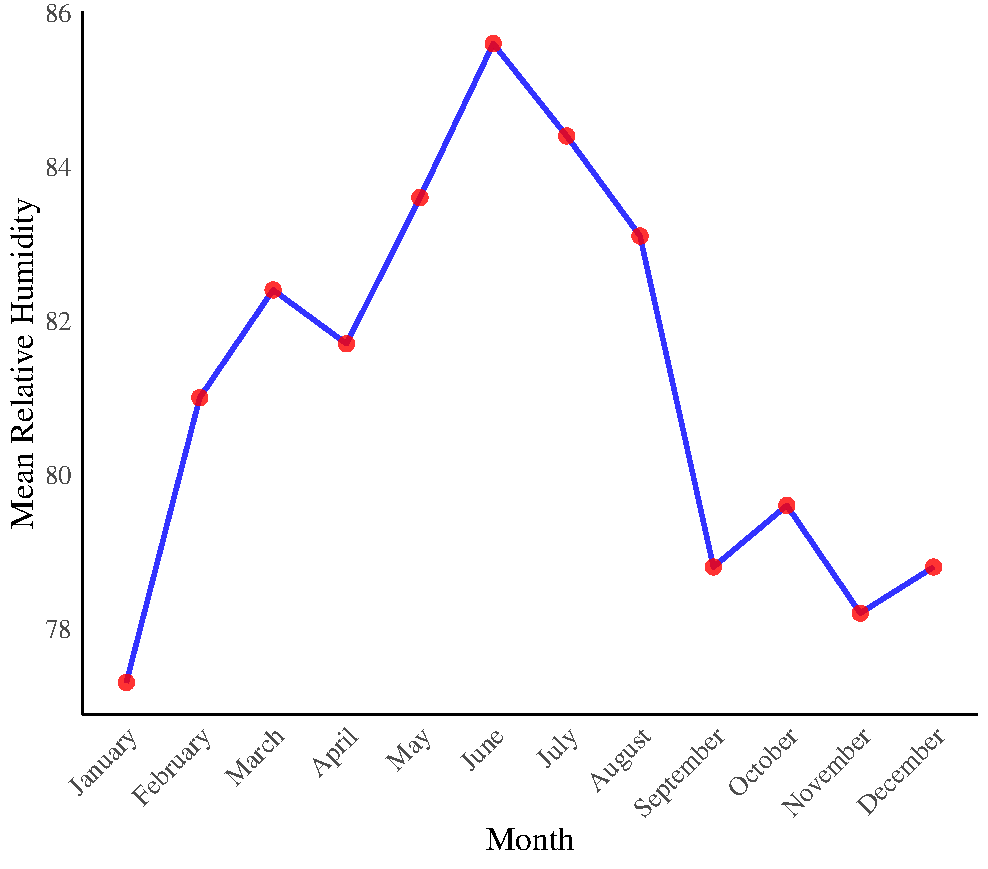
\includegraphics[width=0.6\textwidth]{humidity graph}
	\caption{Mean Monthly humidity in Wellington}
\end{figure}
%%% ACF Remove lines that carry no meaning

We construct the histogram of proportions $h=(h_1,h_2,h_3,h_4,h_5,h_6)$, where each bin $h_l$ represents the proportion of symbols of type $\pi^l$ out of the total six symbols. The histogram graph is shown below.

\begin{figure}[hbt]
	\centering
	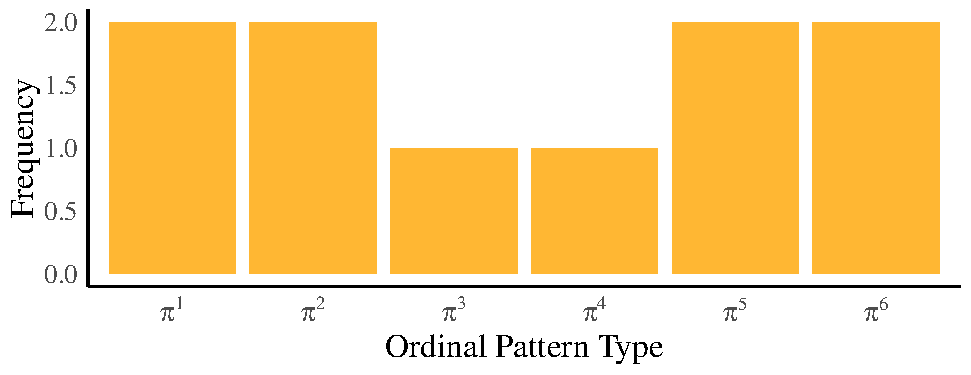
\includegraphics[width=0.6\textwidth]{frequency histogram}
	\caption{Histogram}
\end{figure}

%%% ACF End the section with the briefest possible summary, and an anticipation of what comes next






\chapter{Literature Review}\label{C:lit}

The analysis of complex time series has long relied on both time-domain and frequency-domain techniques. However, traditional methods often fall short in capturing nonlinear dynamics or are limited by strict assumptions such as stationarity and Gaussianity. The ordinal symbolic approach introduced by Bandt and Pompe in 2002 marked a significant theoretical advance by enabling robust, model-free characterization of time series. Their approach, rooted in information theory, involves converting segments of time series data into symbolic patterns based on the ordinal (rank) relationships among data points. The entropy calculated from the distribution of these patterns, now widely known as permutation entropy, has since become a central tool in nonlinear data analysis. This literature review discusses the theoretical foundations and diverse applications of the Bandt-Pompe methodology, as well as recent developments and challenges outlined in contemporary works, including the review by Amigó et al.~\cite{amigo2023ordinal} and Leyva et al.~\cite{Leyva2022}.

%Waschke et al.~\cite{Waschke2025} investigated how the hippocampus encodes sensory information during memory formation by analyzing time series data from single-neuron recordings in 34 human patients undergoing neurosurgical procedures. Using permutation entropy, a measure of temporal complexity, they quantified trial-to-trial variability in neuronal spiking activity during a visual memory task. Their analysis revealed that hippocampal neurons dynamically track the richness of visual input, with greater spiking variability corresponding to more complex or information-rich stimuli. Key features of the study include the use of intracranial single-neuron recordings in humans, the application of entropy-based metrics to capture neural variability, and the discovery that this variability not only reflects stimulus content but also predicts subsequent memory performance, highlighting the role of variability as a functional marker of memory encoding. 

%Another study by Alessio Perinelli and Leonardo Ricci \cite{Perinelli2025} aimed to develop a statistically grounded method to evaluate the temporal stationarity of resting-state EEG data using permutation entropy (PE). Researchers analyzed EEG recordings from the LEMON dataset, involving young and elderly adults, during alternating eyes-open (EO) and eyes-closed (EC) conditions. EEG signals were source-reconstructed into 30 brain regions, segmented, and assessed for entropy-based stability using a chi-square test on PE values. Key findings revealed greater nonstationarity in elderly participants and in EC conditions, with unstable segments showing higher PE, indicating increased signal complexity. This method provides a reliable framework for identifying unstable EEG periods and has potential applications in clinical diagnostics and real-time neural monitoring.

%Li et al.~\cite{Li2025} discussed the Multiscale Grayscale Dispersion Entropy (MGDE) model, an advanced entropy-based metric designed to assess the complexity of time series data across multiple temporal scales. Building upon the foundation of Grayscale Dispersion Entropy (GDE), MGDE incorporates a multiscale framework that enables a more comprehensive analysis of dynamic behaviors in time series. The methodology involves applying a coarse-graining process to the original time series data, followed by the computation of GDE at each scale, effectively capturing the signal's complexity at various temporal resolutions. Key findings from the study demonstrate that MGDE effectively distinguishes between different types of signals, including white Gaussian noise, $1/f$ noise, and chaotic signals, highlighting its robustness and sensitivity to underlying dynamics. The research also emphasizes MGDE's computational efficiency and its potential applicability in real-time signal processing. Looking ahead, MGDE holds significant promise for diverse applications in fields such as biomedical engineering, finance, and environmental science, where understanding the multiscale complexity of time series data is essential.

%The article titled "Detection of Ship Echo Signals in Reverberation Background Based on Sample Entropy and Multiscale Sample Entropy" by Li et al.~\cite{Li2025a}, addresses the challenge of detecting ship echo signals amidst reverberation in underwater environments. Traditional frequency-based detection methods often struggle under conditions of low signal-to-reverberation ratios (SRR) and minimal Doppler shifts. To overcome these limitations, the authors introduce entropy-based approaches, specifically, Sample Entropy (SampEn) and Multiscale Sample Entropy (MSE), to analyze the complexity differences between target echoes and reverberation noise. Through simulations under various SRR and Doppler shift scenarios, the study demonstrates that while frequency-based methods falter in challenging conditions, SampEn and MSE effectively detect target echoes. Notably, MSE maintains detection capabilities even when the Doppler shift is negligible and the SRR drops to 0 dB. These findings highlight the robustness of entropy-based methods in complex underwater acoustic environments, suggesting their potential for enhancing real-time sonar systems and underwater surveillance applications.

%Mao et al.~\cite{Mao2025} introduces an innovative approach for detecting short-wave defects in railway tracks by analyzing axle box acceleration signals. The authors propose a new metric called Dispersion Transition Entropy (DTE), which quantifies the dynamic complexity of time series data by examining transitions between dispersion patterns. To enhance the sensitivity of this measure, they integrate the Jensen–Fisher Divergence (JFD), a statistical tool adept at highlighting local differences in probability distributions. By computing the JFD between dispersion-transition distributions of consecutive sliding windows, the method effectively identifies anomalies such as rail corrugation and impact defects. Experimental results demonstrate that this combined approach outperforms traditional methods in distinguishing chaotic signals from stochastic noise, offering a robust solution for real-time rail defect detection and contributing to improved railway maintenance and safety.

%An innovative entropy-based metric designed to quantify synchrony in complex time series data was proposed by Lin A. and Lin G.~\cite{Lin2025}. The method extends traditional diversity entropy by incorporating a multiscale framework, enabling the analysis of signal complexity across various temporal resolutions. By evaluating the diversity of patterns within time series at multiple scales, the approach captures both local and global synchrony features, making it particularly effective for detecting subtle synchronization phenomena in nonlinear and nonstationary signals. The study demonstrates the utility of this metric through applications to both synthetic and real-world datasets, highlighting its robustness and sensitivity in identifying synchrony patterns that may be overlooked by conventional methods. The findings suggest that multiscale modified diversity entropy offers a valuable tool for researchers and practitioners in fields such as neuroscience, physiology, and engineering, where understanding the synchrony of complex systems is crucial.

%A novel approach based on Fuzzy Diversity Entropy (FDE) to enhance the accuracy and sensitivity of fault detection in rotating machinery was introduced by Jiao et al.~\cite{Jiao2025}. This method builds on traditional Diversity Entropy (DE) by addressing its limitations in detecting subtle signal variations caused by rigid classification boundaries. By integrating fuzzy set theory, FDE replaces fixed probability assignments with fuzzy membership degrees, enabling a more nuanced quantification of signal complexity and better preservation of diversity information. This enhancement allows FDE to effectively distinguish between similar cosine similarity values that DE might treat as equivalent, thus increasing sensitivity to minor signal changes. The effectiveness of FDE was validated using both simulated and experimental vibration signals from rotating machinery. Comparative analyses show that FDE outperforms conventional DE, Fuzzy Entropy (FE), and Permutation Entropy (PE) in terms of complexity quantification, parameter sensitivity, and computational efficiency. These results suggest that FDE is a robust and efficient tool for intelligent fault diagnosis, with strong potential for real-time monitoring and predictive maintenance of rotating machinery systems.

%A novel signal processing framework to enhance the sensitivity and accuracy of quartz-enhanced photoacoustic spectroscopy (QEPAS) systems for gas detection was proposed by Zhang et al.~\cite{Zhang2025}. The method combines Improved Complete Ensemble Empirical Mode Decomposition with Adaptive Noise (ICEEMDAN), Permutation Entropy (PE), and Wavelet Threshold Denoising (WTD) to efficiently extract and denoise key components from complex acoustic signals. By decomposing the signal into intrinsic mode functions (IMFs) with ICEEMDAN, selecting relevant components using PE, and applying WTD to reduce residual noise, the approach significantly boosts the signal-to-noise ratio. Experimental validation shows that this integrated technique outperforms conventional denoising methods, resulting in more accurate gas concentration measurements. The work highlights the potential of advanced entropy-based and multi-stage denoising strategies in improving the performance and reliability of QEPAS systems for applications such as environmental monitoring, industrial safety, and medical diagnostics.

%Wang et al.~\cite{Wang2025} introduces a novel entropy-based approach aimed at enhancing the accuracy of fault detection in rolling bearings. This method, termed Distance Similarity Entropy (DSE), integrates distance metrics with entropy calculations to effectively capture subtle nonlinear characteristics in vibration signals. By quantifying the similarity between signal segments through distance measures and assessing their complexity via entropy, DSE provides a more sensitive feature extraction technique compared to traditional entropy methods. Experimental validations demonstrate that DSE outperforms existing approaches in identifying bearing faults, especially in scenarios with limited or noisy data, highlighting its potential for practical applications in machinery fault diagnosis.

%Fan and Ding~\cite{Fan2025} presents a novel class of three-dimensional discrete memristive chaotic maps (3DDMCM) derived from a discrete cosine memristor model. These maps exhibit unique dynamic behaviors, including the generation of multi-type hidden attractors such as multi-wave, multi-cavity, multi-firework, and multi-diamond patterns, even in the absence of equilibrium points. By adjusting control parameters $\mu$ and $b$, the system can produce various chaotic attractors, demonstrating phenomena akin to multi-scroll patterns. Dynamic analyses reveal that the system possesses two positive Lyapunov exponents, high complexity, offset boosting, and diverse geometric control behaviors. A pseudo-random number generator (PRNG) based on this system was constructed, showcasing desirable statistical properties suitable for secure communication applications. Furthermore, the feasibility of implementing the 3DDMCM was confirmed through deployment on a DSP development board, underscoring its potential for practical engineering applications

\section{Theoretical Foundations of the Bandt-Pompe Methodology}
Bandt and Pompe (2002) \cite{PhysRevLett.88.174102} introduced a novel approach to time series analysis by focusing on the ordinal relationships between data points rather than their actual values. This method involves mapping a time series into a sequence of ordinal patterns, which are permutations representing the relative ordering of values within embedding vectors. The frequency distribution of these patterns forms the basis for calculating Shannon entropy, a measure of complexity that is invariant under monotonic transformations and robust to observational noise. This approach requires minimal assumptions about the data and is computationally efficient, making it suitable for analyzing a wide range of systems \cite{Zanin2012}.

Shannon entropy is employed to quantify the unpredictability or complexity of the symbolic sequence. The resulting permutation entropy has several attractive properties: it is computationally efficient, non-parametric, and effective for short and noisy time series \cite{PhysRevLett.88.174102, Zanin2012}. Further theoretical development by Rosso et al.~\cite{Rosso2007} extended the theoretical basis by introducing statistical complexity, which reflects both randomness and structure in a system. Plotting entropy against complexity yields the entropy-complexity plane, a diagnostic tool for classifying different dynamical regimes.

\section{Applications and Advances}
The Bandt-Pompe framework has since found broad applications across domains, as reviewed by Amigó et al.(2023) in their survey “Ordinal Methods: Concepts, Applications, New Developments and its Challenges”\cite{amigo2023ordinal}. This section is divided into four subsections to analyze the applications of the Bandt and Pompe framework across various domains:

\subsection{Biomedical Signal Processing}
In biomedical signal processing, it has been used to analyze EEG, ECG, and fMRI data, detecting anomalies such as epileptic seizures or sleep stage transitions. 
\begin{itemize}
	\item \textbf{EEG Analysis:} A study by Keller et al.~(2014)\cite{Keller2014} demonstrated the application of ordinal pattern based entropy measures, such as empirical permutation entropy (ePE), empirical conditional entropy (eCE), and robust empirical permutation entropy (rePE) to effectively analyze and classify EEG time series data, demonstrating their utility in detecting brain state transitions, segmenting non-stationary signals, and identifying change-points without relying on prior expert knowledge.
	
	\item \textbf{ECG Analysis:} Mansourian et al. (2024)\cite{Mansourian2024} applied adaptive improved permutation entropy to extract fetal QRS complexes from single-channel abdominal ECG, enhancing the accuracy of fetal heart rate monitoring.
\end{itemize}

\subsection{Geophysics and Hydrology}
In the fields of geophysics and hydrology, PE has been applied to detect climatic variability and hydrological patterns.
\begin{itemize}
	\item \textbf{Climate Variability:}
	
	\item \textbf{Hydrological Patterns:}
\end{itemize}

\subsection{Econophysics, Optical Systems, and Engineering}
Permutation entropy has found applications in econophysics for market behavior analysis, in optical systems for detecting chaos, and in engineering for fault detection and diagnostics.
\begin{itemize}
	\item \textbf{Econophysics:}
	
	\item \textbf{Optical Systems:}
	
	\item \textbf{Engineering:}
\end{itemize}

\subsection{Methodological Extensions}
Recent developments have extended the methodology through multiscale approaches, cross-entropy comparisons for multivariate signals, and weighted ordinal patterns.

 

Furthermore, the use of alternative entropy measures such as Tsallis and Renyi entropy has been explored to better capture non-extensive and multifractal behavior in complex systems.

\section{Challenges and Future Directions}
Despite its success, several challenges remain in the application and development of the Bandt-Pompe approach. One major issue is the choice of embedding parameters (dimension and delay), which significantly affect the pattern distribution. Additionally, estimating entropy and complexity reliably in short time series remains difficult, prompting the need for improved statistical inference methods such as bootstrapping and confidence interval estimation.

Amigó et al.~\cite{amigo2023ordinal} emphasize the need for more robust inferential frameworks, better handling of multivariate and high-dimensional data, and integrating ordinal methods with machine learning for automated pattern recognition. As ordinal symbolic analysis continues to evolve, it holds promise for deeper insights into both theoretical dynamics and real-world systems.

As a final conclusion related to this literature review, the Bandt-Pompe method has become a foundational tool in time series analysis, offering a robust and intuitive approach to understanding complex dynamics. Through the use of ordinal patterns and entropy-based descriptors, researchers can extract meaningful information from noisy, nonlinear, and non-stationary data. While challenges remain, ongoing theoretical advances and applications across disciplines ensure the continued relevance and growth of this methodology.






\chapter{The Research Project}\label{C:aim}

In this chapter, we outline the main ideas and objectives of this research project. 
%%% ACF Only complexity?
Section~\ref{Sec:AdvantagesLimitations} discusses entropy and complexity analysis in time series, highlighting its advantages and limitations. 
%%% ACF Use numbered sections/subsections and refer to their automatic numbers
Section~\ref{Sec:BP method} examines the advantages and  limitations of the Bandt and Pompe method. 
Section~\ref{Sec:BackgroundKnowledge}  provides background knowledge on the 
%%% ACF What is this plane?
entropy-complexity plane. 
Section~\ref{Sec:EntropyComplexity} explores the entropy-complexity plane for a broad class of time series. Section~\ref{Sec:AsymptoticDistribution} provides the asymptotic distribution of the entropy. Finally, the chapter concludes with the objectives of the research project and a case study related to our work.

%%% ACF Do you analyse complexity only?
\section{Entropy and Complexity Analysis in Time Series: Advantages and Limitations}\label{Sec:AdvantagesLimitations}

Entropy and complexity analysis provides powerful tools for characterizing the unpredictability and structural richness of dynamical systems, which evolve over time. Entropy measures, such as Shannon entropy (quantifying uncertainty in a probability distribution) and permutation entropy (which measures the order structure of a time series through ordinal patterns), are widely used to assess randomness and disorder. The main distinction is that permutation entropy computes Shannon entropy on the ordinal patterns extracted from a time series data.
%%% ACF What's the difference between SE and PE?
 

Complexity measures complement entropy by evaluating the balance between order and chaos. Together, entropy and complexity are particularly effective for detecting nonlinear patterns, relationships captured by nonlinear models, where inputs and outputs are not proportional and small changes can produce large or unpredictable effects. Such behavior frequently appears in biological, financial, or climate systems.

%%% ACF What is a nonlinear pattern?

While these methods reveal hidden structures and irregular dynamics beyond the reach of traditional linear approaches, they also require careful preprocessing, appropriate parameter selection (e.g., embedding dimension and time delay), and sufficient domain knowledge. Without this, interpretations may be misleading.


Despite these challenges, entropy and complexity remain essential in modern time series analysis. Unlike linear techniques, such as auto-correlation, regression, or Fourier analysis, that assume proportional and stationary relationships, entropy and complexity measures are designed to capture irregularities, pattern changes, and chaotic dynamics. This makes them invaluable for studying complex and nonlinear systems where conventional tools often fall short.
%%% ACF Several problems with the following sentence. (1) at some point, we will say that OPs are little sensitve to outliers, (2) we don't know what "data length" means
%They can be sensitive to noise and data length. 
%%% ACF Rethink the following assertion. I tend to disagree. Computing these quantities is not computationally intensive; but computing their statistical properties taking into account the serial correlation is
%%% ACF What is a high dimensional system?
%%% ACF What is a multi-scale system?


\section{The Bandt and Pompe Method: A Robust Approach} \label{Sec:BP method}

%%% ACF Reserve "demonstrate" for mathetical proofs
The concept of ordinal patterns in time series can be effectively studied through real world examples. 
Traditionally, numerous algorithms, techniques, and heuristics have been employed to estimate complexity measures from real world data. 
%%% ACF What is a low-dimensional dynamical system? the number of state variables or dimensions are small, we called it as low dimension. 1D, 2D or 3D can be considered as low dimension. 

However, these methods often perform well only for low-dimensional dynamical systems and struggle when noise is introduced. Low-dimensional dynamical systems are systems whose behavior can be described using a small number of variables or equations, typically two or three, such as the logistic map, or pendulum. These systems exhibit rich and often chaotic dynamics but remain mathematically tractable and easier to analyze using entropy and complexity measures. Because of their limited dimensionality, the patterns within the data are more distinct, making it easier to extract meaningful information. 

%%% ACF What is the Lyapunov exponent? It is one of the complexity parameters. It measures how small changes grow over time. 
The Bandt and Pompe method overcomes this limitation by providing a robust approach that remains reliable even in noisy environments. 
In time series analysis, key complexity parameters such as entropy, fractal dimension, 
%%% ACF If you mention it, you must  be able to define it
and Lyapunov exponents play a crucial role in comparing neighboring values and uncovering the underlying structure and dynamics of the data. A Lyapunov exponent measures the average rate at which nearby trajectories in a dynamical system diverge or converge. It provides deeper understanding of system's behavior. 

The advantages of Bandt \& Pompe methods:
\begin{itemize}
	\item Simplicity
	\item Extremely fast calculation
	\item Robustness
	\item Invariance to nonlinear monotonous transformations
\end{itemize}	

This method exhibits low sensitivity to noise and naturally accounts for the causal order of elements in a time series. As a result, it can be applied to various real-world problems, particularly in differentiating between chaotic and stochastic signals.

Despite its limitations, researchers have developed extensions to the original method to address its shortcomings and enhance its applicability to a broader range of complex systems.

\section{Statistical Complexity measures} \label{Sec:BackgroundKnowledge}

Bandt and Pompe introduced a highly effective method for analyzing time series within this framework. They calculated Shannon entropy based on the histogram of causal patterns and successfully identified chaotic components in sequences of words, among other applications.

Later, Rosso et al.~\cite{EEGAnalysisUsingWaveletBasedInformationTools} expanded this analysis by introducing an additional dimension: the statistical complexity derived from the same histogram of causal patterns. The authors have contributed to a wide range of applications. This approach, which utilizes the entropy-complexity plane, has been successfully applied to the visualization and characterization of different dynamical regimes as system parameters change  \cite{Bandt2005,Cao2004,DeMicco2012a,Kowalski2007,Kowalski2011b,Rosso2010a,Zunino2010a,Zunino2012a}, as well as to optical chaos \cite{Liu2016f,Soriano2011a,Toomey2014,Yang2015e,Zunino2011a}, hydrology \cite{Lange2013,Serinaldi2014,Stosic2016}, geophysics \cite{Consolini2014,Saco2010,Sippel2016}, engineering \cite{Aquino2017,Aquino2015,Redelico2017a,Yan2012}, biometrics \cite{Rosso2016}, characterization of pseudo-random number generators \cite{DeMicco2008,DeMicco2009}, biomedical signal analysis \cite{Li2014b,Li2008b,Li2007,Liang2015b,Montani2015a,Montani2014,Montani2014a,Montani2015,Morabito2012,Parlitz2012,Perinelli2025,Perinelli2019,Zanin2012}, and econophysics \cite{Bariviera2015a,Bariviera2015,Bariviera2016,Zanin2012,Zunino2016a,Zunino2009,Zunino2010}, to name a few.

After computing all symbols as described in Chapter~\ref{C:intro}, the histogram proportions are used to estimate the probability distribution of ordinal patterns. 
From this distribution, two key descriptors are calculated to characterize the time series:
\begin{enumerate}
	\item Entropy 
	
	\item Statistical complexity
\end{enumerate}
The most common metric for the first descriptor is the normalized Shannon entropy, defined as:
\begin{equation}
	H(\mathbf{p})=-\dfrac{1}{\log k}\sum^{k}_{\ell=1}p_{\ell} \ln{p_{\ell}}.
\end{equation}
Here, $k=D!$ represents the total number of possible permutation patterns.
%%% ACF Something is missing here
This entropy is bounded within the unit interval:
\begin{itemize}
	\item It reaches its minimum value $(H=0)$ when a single pattern dominates, i.e., $p_{\ell}=1$ for some $\ell$.
	\item It achieves its maximum $(H=1)$ under uniform probability $p_{\ell}=1/k$ for all $\ell$. 
\end{itemize}
This normalized entropy is often termed permutation entropy in time series analysis. 

While normalized Shannon entropy is a powerful tool for quantifying disorder, it fails to fully characterize complex dynamics. To address this limitation, López-Ruiz et al.~\cite{lopez1995statistical} introduced the disequilibrium $Q$ concept, which quantifies the deviation of a probability distribution $\mathbf{p}$ from a uniform (non-informative) equilibrium state. 
%%% ACF Here you say that the disequilibrium is the Euclidean distance, but then you say that it is the Jensen-Shannon
López-Ruiz and the team employed the Euclidean distance between $\mathbf{p}$ and the uniform distribution, providing a complementary metric to Shannon entropy for assessing structural complexity in systems.

%%% ACF Present the statistical complexity in a logical manner
The Jensen-Shannon distance between histogram of proportion $\mathbf{p}$ and the uniform probability function $\mathbf{u}=(1/k, 1/k, \dots, 1/k)$, where $k=D!$ corresponds to the number of possible permutation patterns provides a robust metric for quantifying deviations from uniformity. This distance measure, derived from the symmetric Jensen-Shannon divergence, is particularly suited for analyzing ordinal pattern distributions due to its ability to capture both structural differences and statistical disequilibrium in time series data.
%%% ACF We don't write like this: Here is the formula for $Q'$:
It is defined as:
\begin{equation}
	Q'(\mathbf{p,u})=\sum^k_{\ell=1} p_\ell\log\dfrac{p_\ell}{u_\ell}+u_\ell\log\dfrac{u_\ell}{p_\ell}.
\end{equation}

Lamberti et al. \cite{lamberti2004intensive} proposed Jensen-Shannon distance as a symmetric metric rooted in the Jensen-Shannon divergence. As the reference model, most works consider the uniform distribution $\mathbf{u}=(1/k,1/k, \dots, 1/k)$. The normalized disequilibrium is defined as follows
\begin{equation}
	Q=\dfrac{Q'}{\max{(Q')}},
\end{equation}
where $\max(Q')$ is defined as follows
\begin{equation}
	\max(Q')=-2 \left[\dfrac{k+1}{k}\log(k+1)-2\log(2k)+\log k\right].
\end{equation}

With this, Lamberti et al. \cite{lamberti2004intensive} proposed complexity as a measure of the statistical complexity of the underlying dynamics, which is defined as 
\begin{equation}
	C=HQ,
\end{equation}
where both $H$ and $Q$ are normalized quantities, therefore $C$ is also normalized. 

\section{The Entropy Complexity Plane} \label{Sec:EntropyComplexity}
The entropy-complexity plane is a two-dimensional representation where time series are mapped based on their entropy and statistical complexity. These metrics are derived from ordinal pattern distributions obtained through embedding dimension $D$ that are mapped on histograms of $D!$ bins. 

\subsection{Key Dynamics in the plane}
\begin{enumerate}
	\item Highly Ordered Systems, where the behavior is very predictable, structured, and often repeats in a regular pattern over time.
	
	Example: Strictly monotonic time series.
	\begin{itemize}
		\item Produces a single ordinal pattern $(H=0)$.
		
		\item Maximal disequilibrium (distance from uniform distribution).
		
		\item Maps to $(0,0),$ indicating minimal complexity.
	\end{itemize}
	
	\item Perfectly Random Systems
	
	Example: White noise
	\begin{itemize}
		\item Uniform ordinal pattern distribution $(H=1)$.
		\item Disequilibrium vanishes (distance $=0)$.
		\item Maps to $(1,0),$ reflecting maximal entropy without structural complexity.
	\end{itemize}
\end{enumerate}
The two extreme values are proved by Anteneodo \& Plastino \cite{anteneodo1996some}.
Expressions for the boundaries, derived using geometrical arguments within space configurations, were proposed by Martin et al. \cite{Martin2006}. 
These formulations provide a structured approach to understanding and analyzing the spatial behavior of specific systems or models. The lower boundary is characterized by a smooth curve, whereas the upper boundary consists of $D!-1$ distinct segments. As the embedding dimension $D$ approaches infinity, the upper boundary gradually converges into a smooth curve. 
Example for the entropy complexity plane is shown in Figure \ref{fig:complexity}. Further, ten time series and their points in the $H \times C$ plane for embedding dimension 6 according to our application is shown in Figure \ref{fig:tentimeseries}.

%%% ACF Illustrate the boundaries for D=3,4,5,6

\begin{figure}[H]
	\centering
	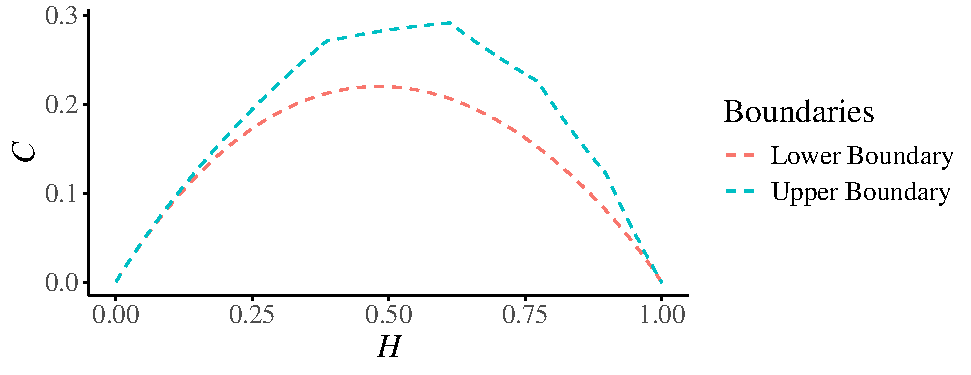
\includegraphics[width=0.7\textwidth]{complexity plane}
	\caption{Entropy Complexity Plane for Embedding dimension 3, 4,5, and 6}
	\label{fig:complexity}
\end{figure}


\begin{figure}[H]
	\centering
	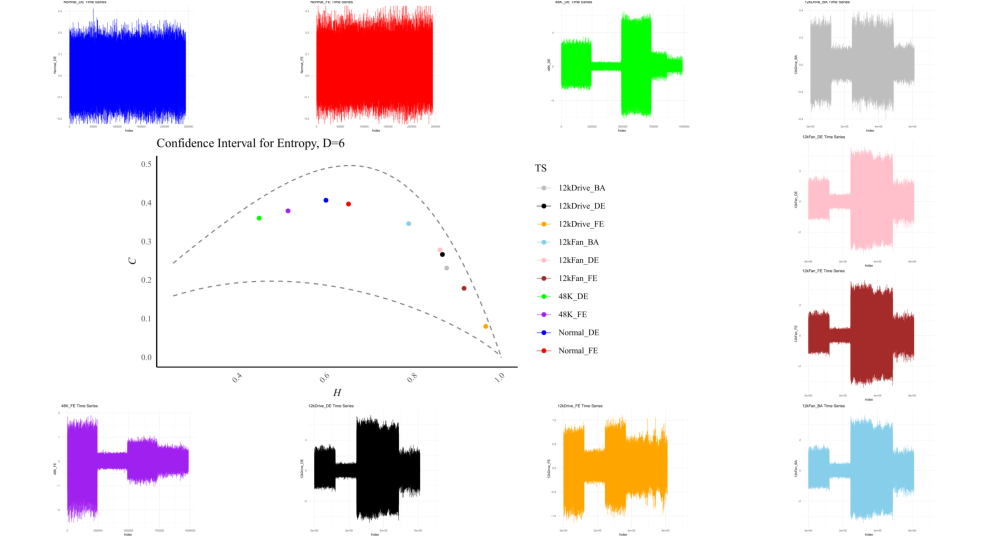
\includegraphics[width=0.7\textwidth]{combined plot}
	\caption{Time series plots and their points in the $H \times C$ plane for Embedding dimension 6}
	\label{fig:tentimeseries}
\end{figure}

\section{Asymptotic Distribution of the permutation entropy}\label{Sec:AsymptoticDistribution}
Ordinal patterns are a robust symbolic transformation method that enables the unveiling of latent dynamics in time series data. This approach involves constructing histograms of patterns and calculating both entropy and statistical complexity. According to the literature, determining the exact distribution of features derived from ordinal patterns is challenging; therefore, researchers have extensively investigated this distribution and its related statistical properties. Two types of statistical distributions are discussed in the literature: the empirical distribution and the asymptotic distribution.

The empirical distribution is used in conjunction with knowledge of the expected variability of entropy and complexity, allowing hypothesis tests to be performed for a wide variety of models according to the underlying dynamics. Results in this direction can be found in the literature~\cite{Chagas2022a, DeMicco2008, Larrondo2005, Larrondo2006}. In this approach, researchers construct empirical distributions directly from observed data, which reflect the actual frequencies of patterns or outcomes.

Furthermore, two types of asymptotic distributions are discussed: the first assumes that patterns are independent and identically distributed (multinomial model), while the second accounts for dependent patterns.

\subsection {Asymptotic Distribution of the Shannon Entropy under the Multinomial Model}\label{Subsec:Multinomial} 

The multinomial distribution models counts of observations in $k$ mutually exclusive categories $\pi^1,\pi^2,\dots,\pi^k$ from $n$ independent trials, with probability vector $\mathbf{p} = (p_1, p_2, \dots, p_k)$, $p_\ell \ge 0$, $\sum_{\ell=1}^k p_\ell = 1$. Let $\mathbf{N} = (N_1, \dots, N_k)$ denote category counts, $\sum_{\ell=1}^k N_\ell = n$. Its probability mass function is
\[
\Pr(\mathbf{N} = \mathbf{n}) = n! \prod_{\ell=1}^k \frac{p_\ell^{n_\ell}}{n_\ell!}, \quad \mathbf{N} \sim \mathrm{Mult}(n, \mathbf{p}),
\]
with moments
\[
E(N_\ell) = n p_\ell, \quad
\mathrm{Var}(N_\ell) = n p_\ell (1-p_\ell), \quad
\mathrm{Cov}(N_\ell, N_j) = -n p_\ell p_j.
\]

The maximum likelihood (ML) estimator $\widehat{p}_\ell = N_\ell / n$ satisfies $n\widehat{\mathbf{p}} \sim \mathrm{Mult}(n,\mathbf{p})$. For any smooth function $g(\mathbf{p})$, the plug-in estimator $\widehat{g}(\mathbf{p}) = g(\widehat{\mathbf{p}})$ is also ML, enabling the asymptotic distribution of Shannon entropy
\begin{equation}
	H(\mathbf{p}) = -\sum_{\ell=1}^k p_\ell \log p_\ell,
	\label{eq:AsymEntropy}
\end{equation}
to be derived from the asymptotic normality of $\widehat{\mathbf{p}}$ as $n \to \infty$.
The Shannon's entropy of a multinomial distributed random variable is bounded between 0 and $\ln k$. The minimum is attained when $p_{\ell}=1$ for some $1\leq \ell \leq k$ and $p_j=0$ for every $j\ne \ell$. The expression is maximized by $p_{\ell}=1/k$ for every $1\leq \ell \leq k$.  

Further, asymptotic distribution can be described as follows. Let $X_n=(X_{1n},X_{2n},\dots,X_{kn})$ be a sequence of independent and identical distributed random vectors, with distribution $\text{Mult}(n,\mathbf{p})$. If $\widehat{\mathbf{p}}$ denotes the vector of sample proportions, and 
\[\mathbf{Y}_n=\sqrt{n}(\widehat{\mathbf{p}}-\mathbf{p})\] 
then
\[E(\mathbf{Y}_n)=\bm 0,\]
\[\text{Cov}(\mathbf{Y}_n)=\mathbf{D_p}-\mathbf{pp}^T,\]
where $\mathbf{D_p}=\text{Diag}(p_1,p_2,\dots,p_k)$, and the superscript $T$ denotes transposition. The asymptotic distribution of $\mathbf{Y}_n$ is multivariate normal with mean vector $\bm 0$ and covariance matrix $\mathbf{D_p}-\mathbf{pp}^T$, denoted as
%%% ACF Check how I wrote it
%The notation for this can be shown as follows.
%
\begin{equation}
	\mathbf{Y}_n \xrightarrow{\mathscr{D}} N(\mathbf{0}, \mathbf{D_p}-\mathbf{pp}^T).
	\label{eq:Cov} 
\end{equation}
 
Our focus is on the statistical properties of $H(\mathbf{p})$ when $\mathbf{p}$ is replaced by its maximum likelihood estimate $\widehat{\mathbf{p}} = (\widehat{p}_1, \widehat{p}_2, \dots, \widehat{p}_k)$. The problem thus reduces to determining the distribution of $H(\widehat{\mathbf{p}})$.

\begin{align}
	H(\widehat{\mathbf{p}})
	&= -\sum_{\ell=1}^k \widehat{p}_\ell \log \widehat{p}_\ell \nonumber \\
	&= -\sum_{\ell=1}^k \frac{N_\ell}{n} \log \frac{N_\ell}{n} \nonumber \\
	&= \log n - \frac{1}{n} \sum_{\ell=1}^k N_\ell \log N_\ell,
\end{align}
under $N=(N_1,N_2,\dots,N_k)\sim \text{Mult}(n,\mathbf{p})$

For the asymptotic distribution case, we refer to the Delta Method theorems and their multivariate version.

\theoremstyle{plain}
\newtheorem{theorem}{Theorem}

\begin{theorem}[Delta Method, univariate]
	Let $X_n$ be a sequence of independent and identically distributed random variables such that 
	$\sqrt{n}(X_n - \theta) \xrightarrow{\mathscr{D}} N(0,\sigma^2)$. 
	Consider a function $h$ such that $h'(\theta)$ exists and $h'(\theta)\neq 0$. 
	Then,
	\[
	\sqrt{n}\,[h(X_n)-h(\theta)] \xrightarrow{\mathscr{D}} N\!\left(0,\,\sigma^2 [h'(\theta)]^2\right).
	\]
\end{theorem}

\begin{theorem}[Delta Method, multivariate]
	Let $\mathbf{X}_n= (X_{1n}, X_{2n}, \dots, X_{kn})$ be a sequence of independent and identically distributed random vectors such that 
	\[
	\sqrt{n}\,(\mathbf{X}_n - \boldsymbol{\theta}) \xrightarrow{\mathscr{D}} N_k(\mathbf{0},\Sigma),
	\]
	where $\boldsymbol{\theta} = (\theta_1,\theta_2,\dots,\theta_k)$ and $\Sigma$ is the covariance matrix. 
	Suppose that $h\colon\mathbb{R}^k \to \mathbb{R}^m$ is continuously differentiable in a neighborhood of $\boldsymbol{\theta}$, with Jacobian matrix
	\[
	B = \left( \frac{\partial h_i}{\partial \theta_j} \right)_{i,j=1}^k,
	\]
	which is non-singular at $\boldsymbol{\theta}$. Then,
	\[
	\sqrt{n}\,\big(h(\mathbf{X}_n)-h(\boldsymbol{\theta})\big) \xrightarrow{\mathscr{D}} N_m\!\left(\mathbf{0},\, B \Sigma B^T\right).
	\]
\end{theorem}

Further, covariance matrix of Equation~\eqref{eq:Cov} can be expressed as 
%%% ACF Use \eqref when referring to equations
%%% ACF Do not leave blank lines between elements of the same sentence
\begin{equation}
	(\mathbf{D_p}-\mathbf{pp}^T)_{\ell j} =
	\begin{cases}
		p_{\ell}(1-p_{\ell}), & \text{if } \ell = j, \\[6pt]
		-\,p_{\ell}p_{j}, & \text{if } \ell \neq j,
	\end{cases}
\end{equation}
for $1\leq {\ell}, j\leq k.$
Even for dependent processes (e.g., Markov chains), normalized Shannon entropy converges to a normal distribution with variance determined by the covariance structure of $\widehat{\mathbf{p}}$. 

Rey et. al.~\cite{Rey2025} derived the asymptotic distribution of statistical complexity, defined as normalized Shannon entropy times normalized Jensen–Shannon divergence from the uniform distribution under the multinomial model. They demonstrated convergence to normality, with variance and bias reflecting the system’s dynamics. Numerical studies confirm robustness even when the multinomial model is approximate, such as in Bandt–Pompe ordinal patterns. 

We refer the asymptotic equation for the mean and variance provided by Rey et. al.~\cite{Rey2025} for our research work.
%%% ACF The following is strange; the left part depends on p, the right-hand side depends on \widehat p: Rasika corrected it
\begin{equation}
	\mu_{n,\widehat{\mathbf{p}}}	= H(\widehat{\mathbf{p}})
	= -\sum_{\ell=1}^k \widehat{p}_\ell \log \widehat{p}_\ell 
	\label{eq:AsympMean}
\end{equation}  

%%% ACF Is the verb missing?
The estimator in~\eqref{eq:AsympMean} is normally distributed with mean $H(\mathbf{p})$ and variance $\sigma^2_{n,\mathbf{p}}$, where
\begin{equation}
	\sigma^2_{n,\mathbf{p}}=\dfrac{1}{n}\sum_{\ell=1}^{k}p_\ell(1-p_\ell)(\log p_\ell+1)^2-\dfrac{2}{n}\sum_{j=1}^{k-1}\sum_{\ell=j+1}^{k}p_\ell p_j(\log p_\ell+1)(\log p_j+1).
\end{equation}


\subsection{Asymptotic distribution of Permutation Entropy under the pattern dependence}\label{Subsec:PatternDependence}

As we discussed earlier, real-valued time series $\mathbf{x}=\{x_1,x_2,\dots,x_{n+D-1}\}$  transform into the series symbols $\mathbf{{\pi}}=({\pi}_1, {\pi}_2,\dots, {\pi}_n)$ from sub-sequences of embedding dimension $D$, where we considered $D!=k$. Due to the overlapping of time windows, the ordinal patterns which we calculate are dependent. 
%%% ACF Use \dots and correct punctuation
For $i=1,2,\dots k$, let $p_i$ be the probability of observing the state $\pi_i$, denote the vector probabilities, $\mathbf{p}={\left\{p_1,p_2,\dots,p_k\right\}}$ and express as $\mathbf{D_p}=\text{Diag}(p_1,p_2, \dots, p_k)$ the diagonal matrix. 
The transition probability of reaching state $\pi_j$ at time 
%%% ACF Is this the same \ell as before? No, I corrected it.
$t+r$ from the state $\pi_i$ at time $t$, for $r=1,2,\dots,D-1$, is denoted by $p^{(r)}_{ij}$. These transition probabilities can be collected in the matrix $\mathbf{Q}^{(r)}$ whose elements are  $p^{(r)}_{ij}$. As describe in the Rey et al.~\cite{Rey2023a} when $n$ is sufficiently large, asymptotic variance of the Shannon entropy defined as follows:

\begin{equation}
	\begin{split}
		\widehat{\nu}^2_{\widehat{\mathbf{p}}} = \widehat{\sigma}^2_{\widehat{\mathbf{p}}} + 
		& \sum_{i=1}^{k}(\log p_i + 1)^2 
		\left[ (2D - 2)p_i^2 + 2\sum_{r=1}^{D-1} \mathbf{Q}^{(r)}_{ii} \right] \\
		& - 2 \sum_{i=1}^{k-1} \sum_{j=i+1}^{k} (\log p_i + 1)(\log p_j + 1) \\
		& \quad \times \left[ (2D - 1)p_i p_j - \sum_{r=1}^{D-1} \left( \mathbf{Q}^{(r)}_{ij} + \mathbf{Q}^{(r)}_{ji} \right) \right].
	\end{split}
	\label{eq:asympvar}
\end{equation} 


%%% ACF The first sentence repeats the last of the previous paragraph: remove the preious content 
%Asymptotic variance of the Shannon entropy of ordinal patterns considering their correlation structure is given in Equation~\ref{eq:asympvar}.
%%% ACF Again, a deterministic quantity does not have a normal distribution: Modified the sentence
For practical purposes, given $n$ sufficiently large, the estimator in~\eqref{eq:AsymEntropy} can be approximated by a normal distribution with mean $H(\widehat{\mathbf{p}})$ and variance $\widehat{\nu}^2_{\widehat{\mathbf{p}}}/n$. In addition, for $\alpha \in (0,1)$ and sufficiently large $n$, the $(1-\alpha)$\SI{100}{\percent} confidence interval for the estimated entropy is given below.

\begin{equation}
  H(\widehat{\mathbf{p}})\pm \dfrac{Z_{\alpha/2}\widehat{\nu}_{\widehat{\mathbf{p}}}}{\sqrt{n}},
  \label{eq:ConfidenceInterval}
\end{equation} 
where $Z_{\alpha/2}$ is the $\alpha/2$-quantile of a standard normal random variable.

For convenience, Equation~\ref{eq:ConfidenceInterval} is referred to and defined as follows.
\begin{equation}
	H(\widehat{\mathbf{p}})\pm \textbf{Semi Length},
	\label{eq:CI}
\end{equation} 
where $\textbf{Semi Length}=\dfrac{Z_{\alpha/2}\widehat{\nu}_{\widehat{\mathbf{p}}}}{\sqrt{n}}$

\subsection{Asymptotic Variance of Statistical Complexity $C(\widehat{\mathbf{p}})$} \label{Subsec:AsympVarComplexity} 
The asymptotic variance of the statistical complexity $C(\widehat{\mathbf{p}})$, under both the multinomial model and dependence, can be expressed using formulas derived for permutation entropy, the Jensen-Shannon divergence, and their joint asymptotics. The key approach follows Rey et al.~\cite{Rey2025} and recent research work by Silbernagel et al.~\cite{silbernagel2025joint} , employing the multivariate Delta method for functions of multinomial proportions.


%%% ACF If it is estimated, it is a constant and its variance is zero: corrected it. 
The variance of the complexity, $C(\widehat{\mathbf{p}})$, has two estimators:
\begin{itemize}
	%%% ACF Provide the expression taking care to make the notation match previous definitions
	\item \textbf{Multinomial model variance}, denoted as $\widehat{\omega}^2_{\widehat{\mathbf{p}}}$, which assumes independent ordinal patterns.
	\item \textbf{Serial dependence variance}, denoted as $\widehat{\eta}^2_{\widehat{\mathbf{p}}}$.
\end{itemize}

\subsubsection{Formula for Asymptotic Variance of Statistical Complexity}
Let:
\begin{itemize}
	\item $\mathbf{p} = (p_1,\dots, p_k):$ ordinal patterns probability vector
	\item $\widehat{\mathbf{p}} = (\widehat{p}_1,\dots, \widehat{p}_k):$ empirical probability vector
	\item $n:$ sample size
	\item $H(\widehat{\mathbf{p}}):$ normalized Shannon entropy
	\item $Q(\widehat{\mathbf{p}}):$ normalized Jensen Shannon divergence from the uniform distribution
	\item $C(\widehat{\mathbf{p}})=H(\widehat{\mathbf{p}}) \times Q(\widehat{\mathbf{p}}):$ normalized statistical complexity
\end{itemize}

\begin{enumerate}
	\item \textbf{Multinomial Model (Independence)}

The estimator is asymptotically normal:
$$ \sqrt{n}(C(\widehat{\mathbf{p}})-C(\mathbf{p})) \xrightarrow{\mathscr{D}} N(\mathbf{0}, \widehat{\omega}^2_{\widehat{\mathbf{p}}}),$$
where the asymptotic variance is 
$$\widehat{\omega}^2_{\widehat{\mathbf{p}}}= \nabla C(\mathbf{p})^T \Sigma \nabla C(\mathbf{p}).$$

\begin{itemize}
	\item $\Sigma =\mathbf{D_p}-\mathbf{p}\mathbf{p}^T$ is the covariance matrix of sample proportions under independence. 
	\item $\nabla C(\mathbf{p})$ is the gradient (vector of partial derivatives) of $C$ with respect to $\mathbf{p}:$
	$$\dfrac{\partial C}{\partial p_\ell}=Q(\mathbf{p})\dfrac{\partial H}{\partial p_\ell}+H(\mathbf{p})\dfrac{\partial Q}{\partial p_\ell},$$
	where: 
	
	\item $\dfrac{\partial H}{\partial p_\ell}=-(\log p_\ell +1),$ 
	\item The exact partial derivative of Jensen-Shannon divergence $Q(\mathbf{p})$ with respect to depends on the definition but can be explicitly calculated.
\end{itemize}


	\item \textbf{Serial Dependence Case} 

For dependent ordinal patterns, the asymptotic variance increases: 
$$\widehat{\eta}^2_{\widehat{\mathbf{p}}} = a \times \widehat{\omega}^2_{\widehat{\mathbf{p}}},$$

where:
\begin{itemize}
	\item 
	$a = \dfrac{\widehat{\nu}^2_{\widehat{\mathbf{p}}}}{\widehat{\sigma}^2_{\widehat{\mathbf{p}}}},$ 
	\item  $\widehat{\nu}^2_{\widehat{\mathbf{p}}}$ is the variance of entropy under serial dependence,
	\item $\widehat{\sigma}^2_{\widehat{\mathbf{p}}}$ is the variance of entropy under independence.
\end{itemize}

%%% ACF Provide the equations
% \item \textbf{Variance Expression for Complexity (Expanded)}
\end{enumerate}
 Bringing these results together:
\[ \text{Var}(C(\widehat{\mathbf{p}})) = \widehat{\eta}^2_{\widehat{\mathbf{p}}} \approx a \nabla C(\mathbf{{p}})^T \Sigma \nabla C(\mathbf{{p}})
\]

\subsection{Other types of Entropy}
%%% ACF At the end of this section, what do we know about them? Any asymptotic result? Under which conditions?

Moreover, other types of descriptors, such as Rényi entropy~\cite{renyi1961measures}, Tsallis entropy~\cite{tsallis1988possible}, and Fisher information~\cite{frieden2004science}, have been proposed to extract additional information that is not captured by Shannon entropy.
From these entropy measures, Fisher information has garnered more attention due to its unique properties. Fisher information is defined as the average logarithmic derivative of a continuous probability density function.

For discrete probability distributions, Fisher information can be approximated by calculating the differences between probabilities of consecutive distribution elements. A key distinction between Shannon entropy and Fisher information lies in their focus: Shannon entropy quantifies the overall unpredictability of a system, while Fisher information measures the rate of change between consecutive observations, making it more sensitive to small changes and perturbations.

The following equations define Tsallis entropy $	(H_{T}^{q}(\widehat{\mathbf{p}}))$, Rényi entropy $(H_{R}^{q}(\widehat{\mathbf{p}}))$, and Fisher information measures $(H_{F}(\widehat{\mathbf{p}}))$ \cite{sanchez2009discrete} :
\begin{equation}
	H_{T}^{q}(\widehat{\mathbf{p}})=\sum_{\ell=1}^{k}\dfrac{\widehat{p_\ell}-\widehat{p_\ell}^q}{q-1},
\end{equation}
where the index $q\in \mathbb{R}\backslash \{1\}$
\begin{equation}
	H_{R}^{q}(\widehat{\mathbf{p}})=\dfrac{1}{1-q} \log \sum_{\ell=1}^{k}{\widehat{p_\ell}}^q,
\end{equation}
where the index $q\in \mathbb{R}^{+}\backslash \{1\}$
\begin{equation}
	H_F(\widehat{\mathbf{p}})=F_0\sum_{\ell=1}^{k-1}\Big(\sqrt{\widehat{p_\ell}_{+1}}-\sqrt{\widehat{p_\ell}}\Big)^2 ,
\end{equation}
where the re-normalization coefficient is $F_0=4$ \cite{sanchez2009discrete}

Rényi entropy, Tsallis entropy, and Fisher information are alternative statistical measures that reveal specific aspects of time-series structure and variability not captured by Shannon entropy. Rey et al. demonstrated that, when computed from empirical ordinal pattern distributions, these measures become increasingly reliable as sample size grows. Specifically, their sample estimates approach well-defined asymptotic distributions that can be used for statistical inference and hypothesis testing.

For the multinomial model, where ordinal patterns are assumed independent and drawn according to fixed probabilities, the sample entropies and Fisher information converge in distribution as $n$ increases: the central limit theorem applies, yielding asymptotic normality for Rényi and Tsallis entropy estimators, as well as for Fisher information. Explicit formulas for mean and variance are available, and confidence intervals can be constructed accordingly. If the empirical histogram is used, these asymptotic results remain valid under large sample size and mild regularity. In all cases, normality holds for entropy-type measures in the multinomial setting, and specific corrections or other distributions (like chi-squared for quadratic forms) may arise for more complex dependency structures. Thus, under the multinomial and empirical frameworks, these advanced entropy and information measures possess robust, predictable properties that enable their practical use in time-series analysis and statistical hypothesis testing.


\section{Case Study of Asymptotic Distribution of the Shannon Entropy under pattern dependence and independence} \label{Sec:CaseStudy} 

Statistical complexity is defined as the product of two normalized quantities:
\begin{itemize}
	\item The Shannon entropy,
	\item The Jensen-Shannon distance between the observed probability distribution and the uniform distribution. 
\end{itemize}

In this section we discuss two key aspects with real world scenario:
\begin{enumerate}
	\item \textbf{Significance of Asymptotic Distributions}: Why understanding large-sample behavior matters for statistical inference,
%	\item \textbf{Multinomial Model Framework}: Derivation of the asymptotic distribution for statistical complexity under Multinomial assumptions
	\item \textbf{Practical Formula}: A working equation for calculating the asymptotic distribution of complexity.
\end{enumerate}

As a case study for our work, we consider data from the Bearing Data Center and the seeded fault test data from Case Western Reserve University, School of Engineering. The datasets includes ball bearing test data for normal bearings as well as single-point defects on the fan end and drive end. Data were collected at a rate of $48,000 (48k$ drive-end) data points per second during bearing tests. Each file contains motor loads $(0, 1, 2,$ and $3)$, drive-end vibration data, and fan-end vibration data. The approximate motor speeds in RPM during testing: $1797, 1772, 1750,$ and $1730$. For our case study, we consider two time series (Normal Baseline and $48k$ Drive-End) with a motor load of $0$ and an RPM of $1797$. 

The primary objective of this study is to detect malfunctioning machinery by analyzing two time series using ordinal patterns. We introduce a distance metric based on the ordinal structure of the segments to quantify similarity. This metric facilitates the identification of faulty machines across various embedding dimensions, ranging from $3$ to $6$. For this case study, we employ an embedding dimension of $3$ for convenience; subsequent analyses will extend to the remaining dimensions to compare results. Permutation entropy under asymptotic conditions is computed by considering the probability distribution of ordinal patterns. The results are further analyzed using the complexity–entropy plane, providing insights into the system's dynamics.

Initially, we analyzed complete datasets from two time series: one comprising 250,000 data points representing the normal baseline at motor load 0, and another containing 2,540,000 data points from the 48k drive end under the same motor load. We computed the entropy and complexity measures for these entire datasets, followed by the calculation of the asymptotic variance as defined in Section~\ref{Subsec:PatternDependence}. This asymptotic variance with pattern independence was then used to determine the confidence interval for entropy (Equation is defined in~\ref{eq:ConfidenceInterval}). The calculation of the semi-length of the interval is given by Equation~\ref{eq:CI}. 
%%% ACF With or without correlation? Justify
The final results are presented in Table~\ref{tab:EnComplexResults}.
%%% ACF Why omitting the standard deviation of the statistical complexity in the table? I did not calculate it for this data set

%%% ACF What is each line?
%%% ACF $\sigma_{\bm{p}}$ is a new notation; moreover, is it an estimate?
\begin{table}[H]
	\centering
	\begin{tabular}{llcr}
		\toprule
		Entropy  & Complexity  & $\widehat{\sigma}_{\widehat{\mathbf{p}}}$ & Semi Length \\
		\midrule
		$0.665235$ & $0.226447$ & $0.358893$ & $0.000441$\\ 
		$0.772973$ & $0.170954$ & $0.324376$ & $0.001287$\\
		\bottomrule
	\end{tabular}
	\caption{Entropy Complexity Results}
	\label{tab:EnComplexResults}
\end{table}

Subsequently, we segmented the data into batches of $10,000$ points, categorizing them as either `Normal` or `48k Drive End`. We then performed a batch wise comparison of entropy and complexity metrics to identify fault data segments. 
The normal dataset comprises $25$ batches, all corresponding to motor load $0$, while the $48k$ drive end dataset includes $254$ batches. Due to the extensive volume of entropy and complexity data generated, the complete results table is not included in this report. However, the entropy–complexity plane effectively illustrates both batch-wise and full-data analyses. As depicted in Figure \ref{fig:EntopyComplexity Plane} below, faulty machines form a distinct cluster in the entropy–complexity plane, highlighting their deviation from normal operational patterns. 
It is clear from the graph that there are both overlapping and non-overlapping confidence intervals. This indicates that some machines differ significantly, while others do not. The main purpose of our experiment is to identify faulty machines. Therefore, we highly recommend extending these results by increasing the embedding dimension to better understand the final outcomes. The general framework of this experiment is also provided in this chapter to clarify the main objective of the research.

\begin{figure}[hbt]
	\centering
	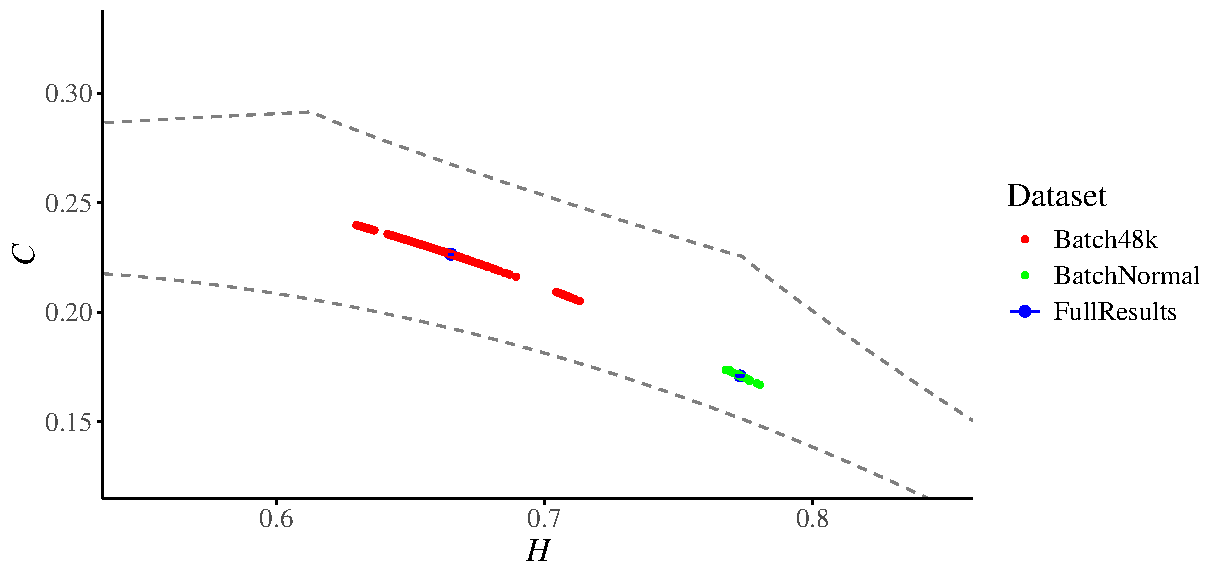
\includegraphics[width=0.8 \textwidth]{confidence_interval}
	\caption{Entropy Complexity Plane}
	\label{fig:EntopyComplexity Plane}
\end{figure}

In addition to this we analyze the full data results for higher embedding dimension $D=6$.
	\begin{figure}[hbt]
	\centering
	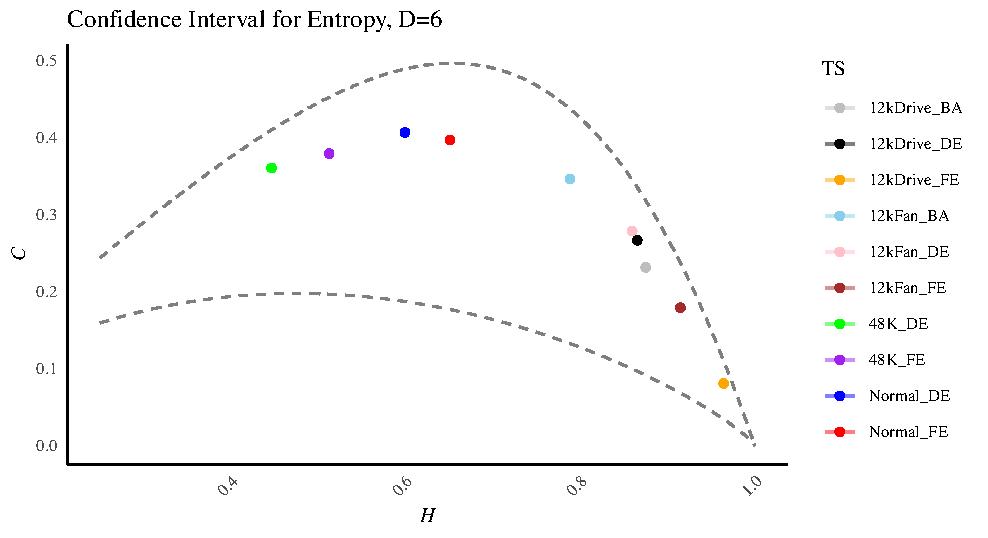
\includegraphics[width=0.8 \textwidth]{Confidence Interval}
	\caption{Entropy Complexity Plane for $D=6$}
	\label{fig:EntopyComplexity Plane D=6}
\end{figure}

Because the original case study involved a large sample size, we computed entropy and statistical complexity for smaller sample sizes of 100, 1000, and 2000. These values were then analyzed using both the Multinomial and Serial Dependence models. The analysis clearly demonstrates the confidence intervals for both entropy and complexity.	

\begin{figure}[H]
	\centering
	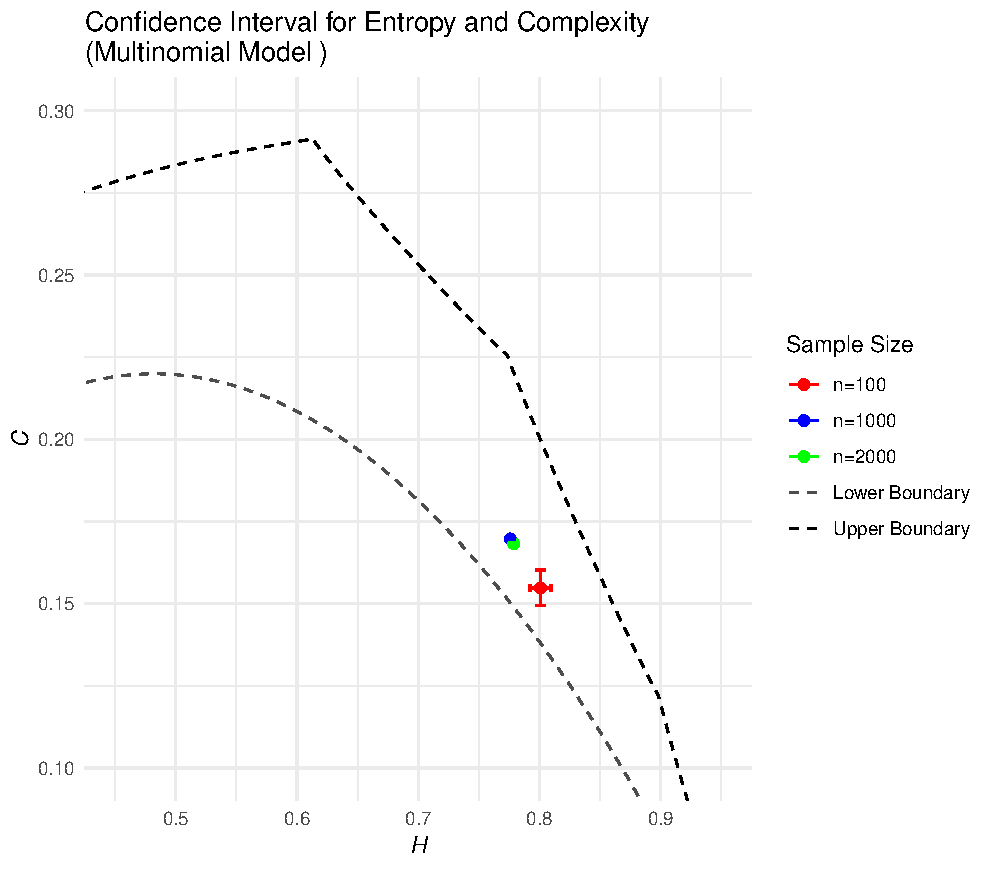
\includegraphics[width=0.8 \textwidth]{CI for Multinomial model}
	\caption{Confidence Interval for Multinomial Model}
	\label{fig:CIMultinorm}
\end{figure}

\begin{figure}[H]
	\centering
	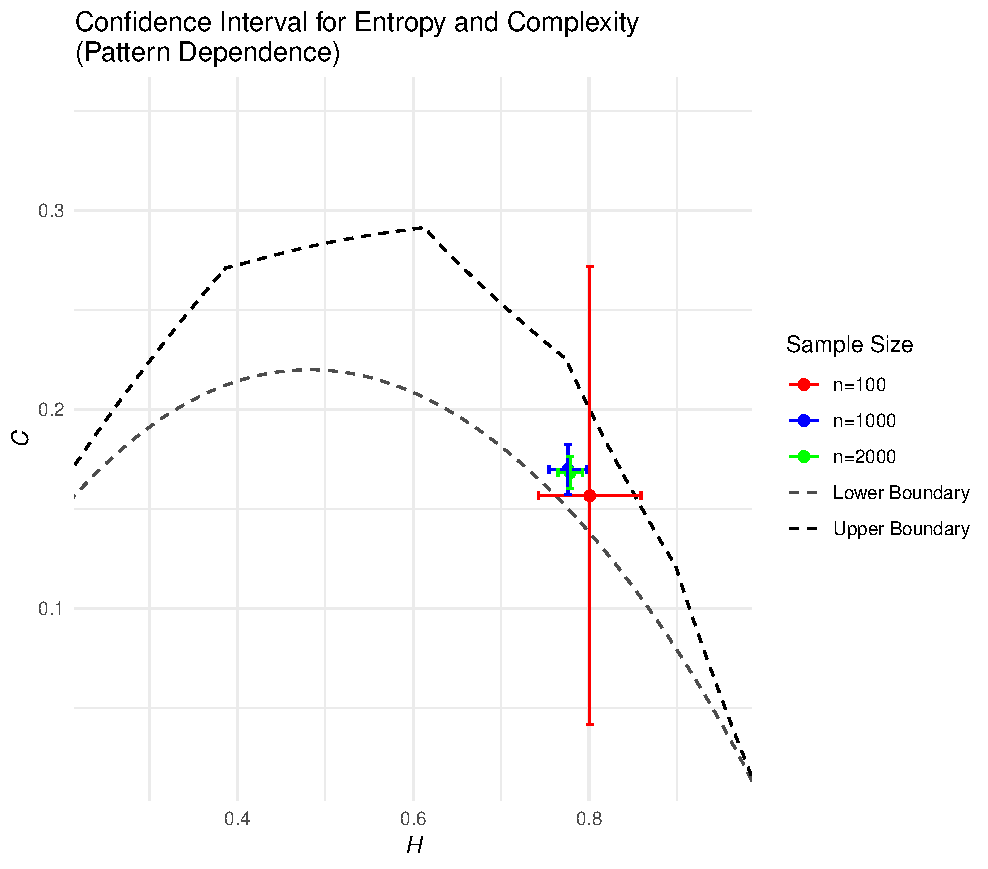
\includegraphics[width=0.7 \textwidth]{CI for pattern dependence}
	\caption{Confidence Interval Pattern Dependence model}
	\label{fig:CIDependence}
\end{figure}

The general framework for analyzing entropy-complexity planes with confidence intervals are given as follows.
\begin{enumerate}
	\item \textbf{Calculate Entropy (H) and Complexity (C):} 
	appropriate estimator are Shannon entropy, statistical complexity measures 
	\item \textbf{Compute Confidence Intervals:}
	Generate multiple resampled datasets to estimate the variance of $H$ and $C$.
	\item \textbf{Plot on Entropy-Complexity Plane:}
	\begin{itemize}
		\item Axes: x-axis: Entropy $(H)$, y-axis: Statistical complexity $(C)$
		\item Data Points: Plot individual or aggregated results.
		\item Confidence Regions: Represent uncertainty 
	\end{itemize}
	
	\item \textbf{Interpretation}
	\begin{table}[H]
		\centering
		\begin{tabular}{cr}
			\toprule
			Region of Plane  & Interpretation  \\
			\midrule
			High $H$ and High $C$ & Complex, structured systems \\ 
			Low $H$ and Low $C$ & Simple, predictable systems \\
			High $H$ and Low $C$ & Random/noisy systems \\
			Low $H$ and High $C$ & Non-random systems \\ 
			\bottomrule
		\end{tabular}
	\end{table}
	
	\item \textbf{Statistical testing:}
	\begin{itemize}
		\item Compare confidence intervals between groups to assess significant differences.
		\item Overlapping intervals $\rightarrow$ {No significant difference}.
		\item Non-overlapping intervals $\rightarrow$ Potential significance.
	\end{itemize}
\end{enumerate}








\chapter{Future Works}\label{C:futw}

As a short summary, we have completed the necessary preliminaries studies on various topics such as:
\begin{itemize}
    \item Entropy
    \item Complexity
    \item Entropy Complexity Plane
    \item Confidence interval
    %\item Multinomial modal.
\end{itemize}

We have also examined key research articles by Bandt and Pompe \cite{PhysRevLett.88.174102}, along with an overview of the area focusing on four seminal works. These include:
\begin{itemize}
	\item López-Ruiz et al. \cite{lopez1995statistical}, who introduced the concept of statistical complexity;
	\item Lamberti et al. \cite{lamberti2004intensive}, who applied López-Ruiz's idea using the Euclidean distance;
	\item Rosso et al. \cite{EEGAnalysisUsingWaveletBasedInformationTools}, who proposed the entropy-complexity plane as a diagnostic tool; and
	\item Martin et al. \cite{Martin2006}, who defined the theoretical boundaries of this generalized statistical complexity measure.
\end{itemize}

In addition, we reviewed recent work by Rey et al. \cite{Rey2025,Rey2023a,Rey2023}, which investigates the statistical properties of entropy derived from ordinal patterns, including the asymptotic distribution under the multinomial law and the behavior of permutation entropy. 

As a case study, we computed the Shannon entropy, statistical complexity, and their associated asymptotic variances based on the probability distribution of ordinal patterns. Using these results, we derived confidence intervals for both entropy and complexity. The analysis was further visualized using the entropy–complexity plane, offering insights into the underlying system dynamics. All computations were performed using two large-sample datasets under the asymptotic distribution, as detailed in Chapter~\ref{C:aim}, Section~\ref{Sec:CaseStudy}. 


The formulas and procedures used to analyze the case study are summarized as follows:
\begin{itemize}
	\item Calculate the Shannon entropy of the time series.
	\item Calculate the statistical complexity.
	\item Estimate the asymptotic variance for Shannon entropy and complexity.
	\item Construct confidence intervals for both entropy and complexity.
	\item Plot the results in the entropy–complexity plane.
	\item Divide the data into batches (batch size = 10,000).
	\item Repeat the above calculations for each batch.
	\item Graphically represent the results of the two time series across batches in the entropy–complexity plane.
	\item Finally, the results are analyzed for time series clustering, as shown in the final output in Figure~\ref{fig:EntopyComplexity Plane}
\end{itemize}


Asymptotic distribution of normalized Shannon entropy $H(\mathbf{p})$ was derived under the assumption of independent ordinal patterns, following the multinomial law. As a foundational step, we use the normalized Shannon entropy formula: 
\begin{equation}
	H(\mathbf{p})=-\dfrac{1}{\log k}\sum^{k}_{\ell=1}p_{\ell} \ln{p_{\ell}}.
\end{equation}
Where, $k=D!$ is the number of possible ordinal patterns. To evaluate statistical complexity, we compute the Jensen–Shannon divergence between the histogram of proportion $\mathbf{p}$ and the uniform probability function $\mathbf{u}=(1/k, 1/k, \dots, 1/k)$, defined by:  
\begin{equation}
	Q'(\mathbf{p,u})=\sum^k_{\ell=1} p_\ell\log\dfrac{p_\ell}{u_\ell}+u_\ell\log\dfrac{u_\ell}{p_\ell}.
\end{equation}

This disequilibrium measure is normalized using:
\begin{equation}
	Q=\dfrac{Q'}{\max{(Q')}},
\end{equation}
where $\max(Q')$ is defined as follows
\begin{equation}
	\max(Q')=-2 \left[\dfrac{k+1}{k}\log(k+1)-2\log(2k)+\log k\right].
\end{equation}

The statistical complexity is then calculated as:
\begin{equation}
	C=HQ,
\end{equation}
where both $H$ and $Q$ are normalized quantities, therefore $C$ is also normalized.   

Then the entropy-complexity plane, which is a two-dimensional representation used to graphically represent the results. 

As a key component of our research, we also calculated the asymptotic variance of the Shannon entropy estimator. The estimated normalized entropy based on sample proportions $\widehat{\bm{p}}$ is: 
\begin{equation}
	H_s(\widehat{\bm{p}})=-\dfrac{1}{\log k}\sum_{\ell=1}^{k}\widehat{p_\ell}\log\widehat{p_\ell}.
\end{equation}

The corresponding asymptotic variance under the multinomial model is given by:
\begin{equation}
	\widehat{\sigma}^2_p=\dfrac{1}{n}\sum_{\ell=1}^{k}p_\ell(1-p_\ell)(\log p_\ell+1)^2-\dfrac{2}{n}\sum_{j=1}^{k-1}\sum_{\ell=j+1}^{k}p_\ell p_j(\log p_\ell+1)(\log p_j+1).
\end{equation}
where $n$ is the sample size. From this variance, we derive confidence intervals for entropy, which are used to assess uncertainty in theentropy-complexity plane. The asymptotic distribution of statistical complexity under the multinomial law is:
\begin{equation}
		C[\widehat{\bm{p}}]=H[\widehat{\bm{p}}]Q[\widehat{\bm{p}}].
\end{equation}

%As defined by Rey et.al.~\cite{Rey2025} the asymptotic distribution of $C[\widehat{\bm{p}}]$ by a normal law, with mean of Shannon entropy ($\mu_C$) and variance (${\sigma}^2_C$)is given by:
%\begin{equation}
%	\mu_C=\dfrac{\max(Q'){\sigma_Q}{\sigma_p}}{n({\delta_Q}{\delta_H}+\rho)},
%\end{equation} 
%\begin{equation}
%	{\sigma}^2_C=\dfrac{{\max(Q')}^2{\sigma^2_Q}{\sigma^2_p}}{{n^2}({\delta^2_Q}+{\delta^2_H}+2\rho \delta_Q \delta_H+1+{\rho}^2)},
%\end{equation}
%where $\rho$ is the correlation coefficient bet ween normalized Shannon entropy and normalized disequilibrium.
%Further, 

%$\delta_Q=\dfrac{n\times \text{asymptotic mean of the Jensen Shannon divergence}(\mu_Q)}{\text{asymptotic variance of disequilibrium}(\sigma_Q)}$,

%$\delta_H=\dfrac{n\times \text{asymptotic mean of the Shannon Entropy}(\mu_C)}{\text{asymptotic variance of Shannon entropy}(\sigma_p)}$.

%Assuming that $n$ is sufficiently large, $\delta_Q$ and $\delta_H$ tend to infinity, we can calculate asymptotic distribution of the complexity.

This approach will be further analyzed, as described in the following objectives, to evaluate the accuracy of the results.

This proposal has three objectives in order to continue this research work.
\begin{itemize}
	\item Define a data base of time series for clustering, i.e., finding similar time series. 
	\item Extract all the features we know from their Bandt \& Pompe symbolization (Shannon, Tsallis and Renyi entropies, Fisher information measure, complexities, and the available confidence intervals)
	\item Use those features for time series clustering 
\end{itemize} 


%\chapter{Statistical Properties of Features from Ordinal Patterns}\label{C:StatisitcalProperty}

Although ordinal pattern based methods, such as permutation entropy, have been widely used for nonlinear time series analysis, the statistical properties of the features derived from these patterns, such as their distribution, variance, and confidence intervals remain under-explored and require further theoretical and empirical investigation. Therefore, the purpose of this chapter is to investigate the researchers who worked related to ordinal patterns, what kind of statistical properties of features used for their research work.

Wang et al.~\cite{Wang2025} uses the Generalized Gaussian Distribution (GGD) as the statistical distribution for its proposed entropy method. This is explicitly stated in their methodology, and the method transforms raw vibration signals using the GGD's Cumulative Distribution Function (CDF) to map data into a normalized space (0 to 1).
Jieren Xie et.al.~\cite{bibid} introduces a novel approach that replaces traditional probability distributions with evidence theory, specifically using belief functions and mass assignments to quantify uncertainty in time series analysis. Instead of relying on fixed probabilities, this method assigns basic probability masses to subsets of permutation patterns, capturing both uncertainty and ignorance through belief intervals. The belief permutation entropy (BPE) is calculated using Deng entropy, which generalizes Shannon entropy by incorporating the cardinality of subsets, allowing for a more flexible representation of uncertainty. This framework integrates neighborhood relationships among permutation patterns, enhancing robustness to noise and ambiguity, particularly in short or non-stationary time series.


	
	
%%%%%%%%%%%%%%%%%%%%%%%%%%%%%%%%%%%%%%%%%%%%%%%%%%%%%%%
	
% and of course book style knows about backmatter
% \backmatter caused problems with appendices :-(
% and of course report style doesn't
%%%%%%%%%%%%%%%%%%%%%%%%%%%%%%%%%%%%%%%%%%%%%%%%%%%%%%%
	
	
%\bibliographystyle{ieeetr}
\bibliographystyle{acm}
\bibliography{BearingFaultDiagnosis}
	
	
\end{document}
